% Paper Psi v3 — Fisher Zeros as Stokes Phenomena
% Author: Grzegorz Olbryk  <g.olbryk@gmail.com>
% March 2026
% Major revision: rigorous proof, 3 clean model demonstrations, theorem paper

\documentclass[12pt]{article}
\usepackage{amsmath,amssymb,amsthm}
\usepackage[margin=2.5cm]{geometry}
\usepackage{hyperref}
\usepackage{booktabs}
\usepackage{graphicx}

\newtheorem{theorem}{Theorem}
\newtheorem{lemma}[theorem]{Lemma}
\newtheorem{proposition}[theorem]{Proposition}
\newtheorem{corollary}[theorem]{Corollary}
\theoremstyle{definition}
\newtheorem{definition}[theorem]{Definition}
\theoremstyle{remark}
\newtheorem{remark}[theorem]{Remark}

\newcommand{\SU}{\mathrm{SU}}
\newcommand{\Tr}{\mathrm{Tr}}
\newcommand{\dU}{\,\mathrm{d}U}
\newcommand{\avg}[1]{\langle #1 \rangle}
\newcommand{\re}{\operatorname{Re}}
\newcommand{\im}{\operatorname{Im}}
\newcommand{\dist}{\operatorname{dist}}
\newcommand{\sgn}{\operatorname{sgn}}

\title{Fisher Zeros as Stokes Phenomena\\of Transfer Matrix Spectra}
\author{Grzegorz Olbryk\\[-2pt]
\small\texttt{g.olbryk@gmail.com}}
\date{March 2026}

\begin{document}
\maketitle

\begin{abstract}
We prove that Fisher zeros of lattice partition functions are
controlled by the Stokes geometry of the transfer matrix spectrum.
For a partition function of the form
$Z_n(s) = \sum_{k=0}^{K} c_k\,e^{n\varphi_k(s)}$,
we establish three results:
(i)~every zero lies within distance $O(n^{-1})$ of the Stokes network
$\mathcal{S} = \{\re\varphi_p = \re\varphi_q\}$;
(ii)~the zero density along each Stokes curve is
$n\,|\dot\theta_p - \dot\theta_q|/(2\pi) + O(1)$;
(iii)~the total zero count in any compact region is
$\mathcal{N} = (n/2\pi)\int_{\mathcal{S}}|d(\theta_p - \theta_q)/dt|\,dt + O(1)$,
linear in~$n$.
We demonstrate the theorem on three models of increasing complexity:
the 1D~Ising model (exact, all zeros on Stokes lines),
the $q$-state Potts model (exact with degeneracy-shifted Stokes curves),
and $\SU(N)$ lattice gauge theory (asymptotic, with shifting
dominant pair).
\end{abstract}


%====================================================================
\section{Introduction}
\label{sec:intro}
%====================================================================

Zeros of the partition function in the complex parameter plane have
been a central tool in the theory of phase transitions since
Yang--Lee~\cite{YangLee1952} and Fisher~\cite{Fisher1965}.  The
distribution of partition function zeros encodes the location and
nature of phase transitions: in the thermodynamic limit, zeros pinch
the real axis at critical points.

Despite extensive numerical study, the \emph{microscopic mechanism}
that generates individual zeros has not been formulated explicitly
for transfer-matrix partition functions.  In this paper we prove that Fisher zeros of
lattice partition functions arise from a universal mechanism: they
are \emph{Stokes phenomena} of the transfer matrix spectrum.

The partition function of an $n$-site system can be written in the
form~\eqref{eq:exp_sum} of Definition~\ref{def:exp_sum} below,
where $\varphi_k(s) = \log A_k(s)$ are complex-valued spectral
exponents (logarithms of transfer matrix eigenvalues), $c_k > 0$
are degeneracies, and~$n$ is the system size.

The key insight is elementary: at any point~$s$ where one exponent
dominates, $Z_n(s) \neq 0$.  Zeros require cancellation, which is
only possible near the \emph{Stokes lines}
$\re\varphi_p(s) = \re\varphi_q(s)$ where two terms compete.

We prove a rigorous theorem (Theorem~\ref{thm:main}) establishing
concentration, density, and counting for zeros of general exponential
sums, then demonstrate it on three models:
\begin{enumerate}
\item The \textbf{1D Ising model} --- an exact two-term sum where
  every zero lies exactly on a Stokes line.

\item The \textbf{$q$-state Potts model} --- an exact two-term sum
  with degeneracy, where zeros lie on an $n$-dependent Stokes curve
  that converges to the asymptotic network.

\item \textbf{$\SU(N)$ lattice gauge theory} --- a multi-term sum
  where zeros concentrate asymptotically on the Stokes network, with
  the dominant pair shifting along the imaginary axis.
\end{enumerate}


%====================================================================
\section{Exponential sums and Stokes networks}
\label{sec:setup}
%====================================================================

\begin{definition}[Exponential sum]\label{def:exp_sum}
A \emph{finite exponential sum of order~$n$} is a function of the form
\begin{equation}\label{eq:exp_sum}
Z_n(s) = \sum_{k=0}^{K} c_k\, e^{n\varphi_k(s)},
\end{equation}
where $K \geq 1$, $c_k > 0$ are positive real coefficients, and
$\varphi_k : \Omega \to \mathbb{C}$ are analytic functions on a
domain $\Omega \subseteq \mathbb{C}$.  We write
$\varphi_k = g_k + i\theta_k$ with $g_k = \re\varphi_k$ and
$\theta_k = \im\varphi_k$.
\end{definition}

\begin{definition}[Stokes network]\label{def:stokes}
The \emph{Stokes network} of~\eqref{eq:exp_sum} is
\[
\mathcal{S} = \bigl\{s \in \Omega : g_p(s) = g_q(s)
\text{ for some } p \neq q\bigr\}
= \bigcup_{p < q} \gamma_{pq},
\]
where $\gamma_{pq} = \{s : g_p(s) = g_q(s)\}$ are the
\emph{Stokes curves}.
\end{definition}

This framework encompasses:

\smallskip
\noindent\textbf{Lattice gauge theories.}
$Z_n(s) = \sum_p d_p\,A_p(s)^n$ with $\varphi_p = \log A_p$,
$c_p = d_p$ (representation dimensions), $s = \kappa + iy$ the
complex coupling, and $n$ the number of plaquettes in the periodic
direction.

\smallskip
\noindent\textbf{1D Ising model.}
$Z_n(\beta) = \lambda_+(\beta)^n + \lambda_-(\beta)^n$ with
$\lambda_\pm = 2\cosh\beta \pm 2\sinh\beta$ and $K = 1$, $c_0 = c_1 = 1$.

\smallskip
\noindent\textbf{$q$-state Potts model.}
$Z_n(\beta) = \lambda_1(\beta)^n + (q{-}1)\,\lambda_2(\beta)^n$ with
$\lambda_1 = e^\beta + q - 1$, $\lambda_2 = e^\beta - 1$, and
$K = 1$, $c_0 = 1$, $c_1 = q - 1$.


%====================================================================
\section{Main theorem}
\label{sec:theorem}
%====================================================================

\subsection{Zero-exclusion lemma}

\begin{lemma}[Zero exclusion]\label{lem:exclusion}
Let $Z_n(s) = \sum_{k=0}^K c_k\,e^{n\varphi_k(s)}$ with $c_k > 0$
and $K \geq 1$.  If there exists $p^*$ such that
\begin{equation}\label{eq:dominance}
c_{p^*}\,e^{n\,g_{p^*}(s)} > \sum_{k \neq p^*} c_k\,e^{n\,g_k(s)},
\end{equation}
then $Z_n(s) \neq 0$.
\end{lemma}

\begin{proof}
Write $Z_n = c_{p^*} e^{n\varphi_{p^*}} (1 + R)$ where
\[
R = \sum_{k \neq p^*} \frac{c_k}{c_{p^*}}\, e^{n(\varphi_k - \varphi_{p^*})}.
\]
Then $|R| \leq \sum_{k \neq p^*} (c_k/c_{p^*})\,e^{n(g_k - g_{p^*})}
< 1$ by hypothesis.  Hence $|1 + R| \geq 1 - |R| > 0$.
\end{proof}

\begin{corollary}[Concentration set]\label{cor:stokes}
Define $\varepsilon_n = n^{-1}\log(K\,c_{\max}/c_{\min})$ where
$c_{\max} = \max_k c_k$ and $c_{\min} = \min_k c_k$.  Every zero of
$Z_n$ lies in
\begin{equation}\label{eq:Sn}
\mathcal{S}_n = \bigl\{s \in \Omega : \exists\, p \neq q \text{ with }
|g_p(s) - g_q(s)| < \varepsilon_n\bigr\}.
\end{equation}
\end{corollary}

\begin{proof}
If $s \notin \mathcal{S}_n$, there is a unique maximiser $p^*$ of
$g_k(s)$ with $g_{p^*} - g_k \geq \varepsilon_n$ for all
$k \neq p^*$.  Then
\[
\sum_{k \neq p^*} c_k\,e^{n g_k} \leq K\,c_{\max}\,e^{n(g_{p^*} - \varepsilon_n)}
= K\,c_{\max}\cdot\frac{c_{\min}}{K\,c_{\max}}\cdot e^{n g_{p^*}}
= c_{\min}\,e^{n g_{p^*}}
\leq c_{p^*}\,e^{n g_{p^*}},
\]
so~\eqref{eq:dominance} holds and $Z_n(s) \neq 0$ by
Lemma~\ref{lem:exclusion}.
\end{proof}

\subsection{Stokes concentration theorem}

\begin{theorem}[Stokes concentration]\label{thm:main}
Let $Z_n(s) = \sum_{k=0}^K c_k\,e^{n\varphi_k(s)}$ be an exponential
sum as in Definition~\ref{def:exp_sum}, and let
$\Omega \subset \mathbb{C}$ be a compact set.  Assume:
\begin{enumerate}
\item[\textup{(A1)}] \textbf{Non-degeneracy:}
  For each pair $(p,q)$ with $\gamma_{pq} \cap \Omega \neq \emptyset$,
  the gradient $\nabla(g_p - g_q)$ does not vanish on
  $\gamma_{pq} \cap \Omega$.

\item[\textup{(A2)}] \textbf{Pairwise dominance:}
  Triple crossings $\{s : g_p = g_q = g_r\}$ in $\Omega$ are
  isolated points (finitely many).

\item[\textup{(A3)}] \textbf{Velocity separation:}
  Along each Stokes curve $\gamma_{pq}$, the phase difference
  $\theta_p - \theta_q$ is non-constant: for any monotone
  parametrisation~$t$ of $\gamma_{pq}$,
  $d(\theta_p - \theta_q)/dt \neq 0$.
\end{enumerate}
Let $\{s_j^{(n)}\}$ be the zeros of $Z_n$ in $\Omega$.  Then:

\begin{enumerate}
\item[\textup{(i)}] \textbf{Concentration.}
Every zero satisfies
\[
\dist\bigl(s_j^{(n)},\, \mathcal{S}\bigr) \leq \frac{C}{n},
\]
where $C = C(\{c_k\}, \{\varphi_k\}, \Omega)$ is independent of~$n$.

\item[\textup{(ii)}] \textbf{Density.}
For each Stokes curve $\gamma_{pq} \subset \mathcal{S} \cap \Omega$,
parametrised by arc length~$t$, the zero density satisfies
\[
\frac{d\mathcal{N}}{dt}\bigg|_{\gamma_{pq}} =
\frac{n}{2\pi}\,\bigg|\frac{d(\theta_p - \theta_q)}{dt}\bigg| + O(1).
\]
In particular, if $\gamma_{pq}$ is parametrised by
$y = \im s$, the density is
$n\,|\dot\theta_p - \dot\theta_q|/(2\pi) + O(1)$.

\item[\textup{(iii)}] \textbf{Counting.}
The total number of zeros in $\Omega$ satisfies
\[
\mathcal{N}(\Omega) = \frac{n}{2\pi} \sum_{j=1}^{J}
\int_{\gamma_{p_j q_j} \cap \Omega}
\bigg|\frac{d(\theta_{p_j} - \theta_{q_j})}{dt}\bigg|\,dt
\;+\; O(1),
\]
where the sum runs over the $J$ Stokes curves in
$\mathcal{S} \cap \Omega$ and $t$ is arc length.
In particular, $\mathcal{N}(\Omega) = O(n)$.
\end{enumerate}
\end{theorem}

\begin{proof}
\textbf{Part~(i): Concentration.}
By Corollary~\ref{cor:stokes}, every zero of $Z_n$ lies in the set
$\mathcal{S}_n$ defined in~\eqref{eq:Sn}, with width parameter
$\varepsilon_n = n^{-1}\log(Kc_{\max}/c_{\min})$.  We must show that
$\mathcal{S}_n$ lies within an $O(n^{-1})$ tube around~$\mathcal{S}$.

Fix a pair $(p,q)$ and consider the real-valued analytic function
$f(s) = g_p(s) - g_q(s)$.  The Stokes curve $\gamma_{pq}$ is the
zero set $\{f = 0\} \cap \Omega$.  By assumption~(A1),
$|\nabla f| \geq m_{pq} > 0$ on $\gamma_{pq} \cap \Omega$.
Since $\Omega$ is compact and $\nabla f$ is continuous, there exists
a neighbourhood $U_{pq} \supset \gamma_{pq} \cap \Omega$ on which
$|\nabla f| \geq m_{pq}/2$.

For any $s \in U_{pq}$ with $|f(s)| < \varepsilon_n$, the mean value
inequality gives
\[
|f(s)| \geq |f(s) - f(\bar s)| \cdot 0 + |\nabla f|_{\min} \cdot
\dist(s, \gamma_{pq}),
\]
where $\bar s$ is the nearest point on $\gamma_{pq}$.  More precisely,
let $\bar s \in \gamma_{pq}$ minimise $|s - \bar s|$, and let
$\mathbf{n}$ be the unit normal to $\gamma_{pq}$ at $\bar s$.  Then
\[
f(s) = f(\bar s) + \langle \nabla f(\bar s), s - \bar s \rangle
+ O(|s - \bar s|^2)
= \langle \nabla f(\bar s), s - \bar s \rangle + O(|s-\bar s|^2).
\]
Since $\nabla f(\bar s)$ is normal to $\gamma_{pq}$ (as
$f|_{\gamma_{pq}} = 0$) and $|\nabla f(\bar s)| \geq m_{pq}$:
\[
|f(s)| \geq m_{pq}\,\dist(s, \gamma_{pq}) - L\,\dist(s, \gamma_{pq})^2,
\]
where $L = \sup_{U_{pq}} \|D^2 f\|/2$.  For $\dist(s, \gamma_{pq})$
sufficiently small (namely, $< m_{pq}/(2L)$), the linear term
dominates, giving
\[
\dist(s, \gamma_{pq}) \leq \frac{2\,|f(s)|}{m_{pq}}
\leq \frac{2\varepsilon_n}{m_{pq}} = \frac{2\log(Kc_{\max}/c_{\min})}{m_{pq}\,n}.
\]

The condition $\dist < m_{pq}/(2L)$ is satisfied for all sufficiently
large $n$ (specifically, $n > 4L\log(Kc_{\max}/c_{\min})/m_{pq}^2$).
For finitely many $n$ below this threshold, the bound
$\dist \leq \mathrm{diam}(\Omega)$ is trivially $O(1) = O(n^{-1})$.

Taking
\[
C = \max_{(p,q)}\, \frac{2\log(Kc_{\max}/c_{\min})}{m_{pq}}
\]
over all pairs $(p,q)$ with $\gamma_{pq} \cap \Omega \neq \emptyset$
gives $\dist(s_j^{(n)}, \mathcal{S}) \leq C/n$ for all~$n$.

Near a triple crossing $s^* \in \gamma_{pq} \cap \gamma_{pr}$, the
zero may approach both curves simultaneously; but since triple
crossings are isolated~(A2), this only affects finitely many points
and does not change the bound.

\medskip
\textbf{Part~(ii): Density.}
Fix a Stokes curve $\gamma_{pq}$ and a point $s_0 \in \gamma_{pq}$
away from triple crossings.  Near $s_0$, the terms $c_p e^{n\varphi_p}$
and $c_q e^{n\varphi_q}$ dominate~$Z_n$; all other terms are
exponentially suppressed:
\[
\delta := \min_{k \neq p,q}\,\bigl(g_p(s_0) - g_k(s_0)\bigr) > 0.
\]

Define the two-term approximation
\[
Z_n^{(2)}(s) = c_p\,e^{n\varphi_p(s)} + c_q\,e^{n\varphi_q(s)},
\]
and the remainder $R_n = Z_n - Z_n^{(2)}$.  On $\gamma_{pq}$,
$g_p = g_q$, so
\[
|R_n| \leq (K{-}1)\,c_{\max}\,e^{n(g_p - \delta)}
\quad\text{while}\quad
|Z_n^{(2)}| \leq 2\,c_{\max}\,e^{ng_p}.
\]
Hence $|R_n|/|Z_n^{(2)}| \leq ((K{-}1)/2)\,e^{-n\delta} \to 0$
exponentially.

The zeros of $Z_n^{(2)}$ satisfy
\begin{equation}\label{eq:2term_zero}
c_p\,e^{n\varphi_p} + c_q\,e^{n\varphi_q} = 0
\quad\Longleftrightarrow\quad
\begin{cases}
n(g_p - g_q) = \log(c_q/c_p), \\[3pt]
n(\theta_p - \theta_q) = (2m+1)\pi.
\end{cases}
\end{equation}
The first equation defines a curve $\tilde\gamma_{pq}^{(n)}$
(the \emph{exact Stokes curve}) at distance $|\log(c_q/c_p)|/(n\,m_{pq})$
from $\gamma_{pq}$, confirming Part~(i) for the two-term zeros.
The second equation, combined with assumption~(A3), gives zeros at
positions along $\tilde\gamma_{pq}^{(n)}$ where
\begin{equation}\label{eq:ym}
\theta_p(s_m) - \theta_q(s_m) = \frac{(2m+1)\pi}{n},
\qquad m \in \mathbb{Z}.
\end{equation}
Parametrising by arc length $t$ along $\tilde\gamma_{pq}^{(n)}$,
the mean value theorem gives consecutive zeros separated by
\begin{equation}\label{eq:spacing}
\frac{d(\theta_p - \theta_q)}{dt}\bigg|_{\xi_m}\,\Delta t_m
= \frac{2\pi}{n},
\end{equation}
so $\Delta t_m = 2\pi/(n\,|d(\theta_p - \theta_q)/dt|) + O(n^{-2})$.
The zero density per unit arc length is
$n\,|d(\theta_p - \theta_q)/dt|/(2\pi)$.

It remains to show that $Z_n$ has the same zeros (up to $O(1)$
corrections) as $Z_n^{(2)}$.  By Rouch\'e's theorem: on a circle of
radius $r = \varepsilon/(n|\varphi_p' - \varphi_q'|)$ centred at each
two-term zero~$y_m$ (with $\varepsilon$ small and fixed), we have
$|Z_n^{(2)}| \geq c_{\min}\,e^{ng_p}\sin\varepsilon > 0$ on the
circle boundary, while $|R_n| \leq (K{-}1)c_{\max}\,e^{n(g_p-\delta)}$.
For $n$ sufficiently large that
$(K{-}1)(c_{\max}/c_{\min})\,e^{-n\delta}/\sin\varepsilon < 1$,
Rouch\'e's theorem guarantees that $Z_n$ has exactly one zero in each
such circle.  There are no other zeros of $Z_n$ between the circles,
because in the gaps, $|Z_n^{(2)}|$ is bounded below by
$c_{\min}\,e^{ng_p}\sin\varepsilon'$ (with $\varepsilon' > 0$) while
$|R_n|$ is still exponentially small.

Thus the zero density of $Z_n$ along $\gamma_{pq}$ equals that of
$Z_n^{(2)}$ up to an $O(1)$ error from boundary effects and
finitely many $n$ below the Rouch\'e threshold:
\[
\frac{d\mathcal{N}}{dt}\bigg|_{\gamma_{pq}} =
\frac{n}{2\pi}\,\bigg|\frac{d(\theta_p - \theta_q)}{dt}\bigg| + O(1).
\]

\medskip
\textbf{Part~(iii): Counting.}
By assumption~(A2), $\mathcal{S} \cap \Omega$ consists of finitely
many smooth Stokes curves $\gamma_{p_1 q_1}, \ldots, \gamma_{p_J q_J}$
(plus isolated triple-crossing points which contribute $O(1)$ zeros).
Each curve has finite arc length in~$\Omega$.  By Part~(i),
every zero of $Z_n$ lies within $O(n^{-1})$ of some~$\gamma_{p_j q_j}$,
and the Rouch\'e correspondence of Part~(ii) assigns each zero
to a unique Stokes curve.  Integrating the density from Part~(ii)
along each curve:
\[
\mathcal{N}(\Omega) = \sum_{j=1}^J
\frac{n}{2\pi}\int_{\gamma_{p_j q_j} \cap \Omega}
\bigg|\frac{d(\theta_{p_j} - \theta_{q_j})}{dt}\bigg|\,dt
\;+\; O(1),
\]
where the $O(1)$ accounts for boundary effects, triple crossings,
and finitely many small~$n$.
Since each integrand is bounded on~$\Omega$ and each curve has finite
arc length, every summand is $O(n)$, giving
$\mathcal{N}(\Omega) = O(n)$.
\qedhere
\end{proof}

\begin{remark}[Sharpness of $O(n^{-1})$]\label{rem:sharpness}
For two-term sums with $c_p \neq c_q$, the exact zeros lie at distance
$|\log(c_q/c_p)|/(n\,m_{pq})$ from $\mathcal{S}$, showing that the
$O(n^{-1})$ bound is sharp.  For $c_p = c_q$ (as in the Ising model),
the zeros lie exactly on $\mathcal{S}$ for all~$n$.
\end{remark}

\begin{remark}[Spacing law]
The spacing between consecutive zeros along a Stokes curve is
\begin{equation}\label{eq:spacing_law}
\Delta y = \frac{2\pi}{n\,|\dot\theta_p - \dot\theta_q|}
+ O(n^{-2}).
\end{equation}
For a model with characteristic spacing constant $C_f$, we have
$\avg{\Delta y} = C_f/n$ where
$C_f = \bigl\langle 2\pi/|\dot\theta_p - \dot\theta_q|
\bigr\rangle_{\text{crossings}}$.
\end{remark}


\subsection{Extension to infinite sums}

The theorem above applies to finite sums.  Many physical partition
functions --- notably lattice gauge theories --- involve infinitely
many transfer matrix eigenvalues.  The following extension closes
this gap.

\begin{proposition}[Tail truncation]\label{prop:tail}
Let $Z_n(s) = \sum_{k=0}^{\infty} c_k\,e^{n\varphi_k(s)}$ be a
series converging absolutely and uniformly on a compact set
$\Omega \subset \mathbb{C}$ for every $n \geq 1$.  Suppose there
exist $K \in \mathbb{N}$, $B > 0$, and $\alpha > 0$ such that
the tail satisfies
\begin{equation}\label{eq:tail_bound}
\bigg|\sum_{k > K} c_k\,e^{n\varphi_k(s)}\bigg|
\leq B\,e^{n\bigl(g_*(s) - \alpha\bigr)}
\quad\text{for all } s \in \Omega,\; n \geq 1,
\end{equation}
where $g_*(s) = \max_{0 \leq j \leq K} \re\varphi_j(s)$.
Then the conclusions of Theorem~\textup{\ref{thm:main}} hold
for $Z_n$ with the $K$-term Stokes network
$\mathcal{S} = \bigl\{\re\varphi_p = \re\varphi_q :
0 \leq p, q \leq K\bigr\}$,
and all error bounds acquire an additional $O(e^{-n\alpha})$
correction.
\end{proposition}

\begin{proof}
Write $Z_n = Z_n^{(K)} + R_n^{(K)}$ where
$Z_n^{(K)} = \sum_{k=0}^K c_k e^{n\varphi_k}$ and
$|R_n^{(K)}| \leq B\,e^{n(g_* - \alpha)}$.

\textup{(i)} The exclusion lemma requires
$c_{p^*} e^{ng_{p^*}} > \sum_{k \neq p^*} c_k\,e^{ng_k}$.
For $Z_n$, the right-hand side gains the tail
$|R_n^{(K)}| \leq B\,e^{n(g_* - \alpha)}$, which is exponentially
small relative to the dominant term $c_{p^*}\,e^{ng_{p^*}}$
(since $g_{p^*} \leq g_*$ and the tail decays as~$e^{-n\alpha}$).
For $n$ large enough that $B\,e^{-n\alpha} < c_{\min}$,
the finite-sum bound applies with an $O(e^{-n\alpha})$ correction.

\textup{(ii)} In the Rouch\'e argument, the remainder
$R_n = Z_n - Z_n^{(2)}$ gains the tail, but on the boundary of
each Rouch\'e circle,
$|Z_n^{(2)}| \geq c_{\min}\,e^{ng_p}\sin\varepsilon$
while $|R_n^{(K)}| \leq B\,e^{n(g_p - \alpha)}$.  The ratio
$|R_n^{(K)}|/|Z_n^{(2)}| \leq (B/c_{\min}\sin\varepsilon)\,
e^{-n\alpha} \to 0$,
so Rouch\'e's theorem still applies.

\textup{(iii)} Follows from~(ii) by integration.
\end{proof}

\begin{remark}[Verification for lattice gauge theories]\label{rem:gauge_tail}
For Wilson-type actions with $S = s\,\re\Tr U$, the transfer matrix
eigenvalues satisfy $A_p(\kappa) \sim (eN\kappa/2p)^p$ for
large~$p$ at real coupling~\cite{OlbrykChi}, giving
super-exponential decay.
For complex coupling, $e^{s\,\re\Tr U}$ is analytic on the compact
group~$\SU(N)$, so the Peter--Weyl coefficients decay exponentially
in the highest weight (cf.~the Paley--Wiener theorem for compact
groups~\cite{Sugiura1990}), suggesting that the tail
bound~\eqref{eq:tail_bound} holds uniformly on compact subsets of
the $s$-plane.  A complete proof of this uniform bound will be given
in~\cite{OlbrykChi}.
Numerically, the 2-term approximation error drops below $10^{-4}$
by $n = 20$ (Table~\ref{tab:large_n}), confirming the rapid tail
decay in practice.
\end{remark}


%====================================================================
\section{Ising model: exact illustration}
\label{sec:ising}
%====================================================================

The 1D Ising model provides the cleanest illustration of
Theorem~\ref{thm:main} because it is an exact two-term sum with
equal coefficients, admitting a closed-form solution.

\subsection{Transfer matrix eigenvalues}

The transfer matrix $T = \bigl[\begin{smallmatrix}
e^\beta & e^{-\beta} \\ e^{-\beta} & e^\beta
\end{smallmatrix}\bigr]$ has eigenvalues
$\lambda_\pm = 2\cosh\beta \pm 2\sinh\beta$, giving
\begin{equation}\label{eq:Z_ising}
Z_n(\beta) = \lambda_+(\beta)^n + \lambda_-(\beta)^n,
\end{equation}
an exponential sum with $K = 1$ and $c_0 = c_1 = 1$.

\subsection{Stokes lines}

At complex coupling $\beta = \beta_r + iy$, the Stokes condition
$|\lambda_+| = |\lambda_-|$, i.e.\ $|\cosh\beta| = |\sinh\beta|$,
reduces to $\cos(2y) = 0$, giving
\begin{equation}\label{eq:ising_stokes}
y_{\text{Stokes}} = \frac{\pi}{4} + \frac{k\pi}{2},
\qquad k \in \mathbb{Z},
\end{equation}
\emph{independent} of $\beta_r$.  These are horizontal lines in the
complex $\beta$-plane.

\subsection{Exact zero formula}

Since $c_0 = c_1 = 1$, the zero condition~\eqref{eq:2term_zero}
requires $|\lambda_+| = |\lambda_-|$ (exactly the Stokes condition)
and $n(\theta_+ - \theta_-) = (2m+1)\pi$.  Equivalently,
$(\coth\beta)^n = -1$.  The solutions are
\begin{equation}\label{eq:ising_zeros}
\beta_k = \frac{1}{2}\log\!\left(\cot\frac{(2k{+}1)\pi}{2n}\right)
\pm \frac{i\pi}{4},
\qquad k = 0, 1, \ldots, \lfloor n/2 \rfloor - 1.
\end{equation}
\emph{Every} zero has $\im\beta = \pm\pi/4$, placing it
\emph{exactly} on a Stokes line~\eqref{eq:ising_stokes}.  This is
the sharpest possible case of Theorem~\ref{thm:main}(i): the
concentration distance is exactly zero, not merely $O(n^{-1})$,
because $c_0 = c_1$.

\subsection{Zero density along Stokes lines}

The zeros~\eqref{eq:ising_zeros} are distributed along the
horizontal Stokes lines.  Parametrising $\gamma$ by
$\beta_r = \re\beta$ (arc length along the horizontal line), the
density from Part~(ii) of Theorem~\ref{thm:main} becomes
\[
\frac{d\mathcal{N}}{d\beta_r} =
\frac{n}{2\pi}\,\bigg|
\frac{d\arg(\coth\beta)}{d\beta_r}\bigg|_{\!y = \pi/4}
+ O(1).
\]
Table~\ref{tab:ising_zeros} verifies the exact formula.

\begin{table}[h]
\centering
\caption{Ising zeros from exact formula~\eqref{eq:ising_zeros},
  all on Stokes line $y = -\pi/4$.}
\label{tab:ising_zeros}
\begin{tabular}{ccccc}
\toprule
$n$ & \#zeros per Stokes line & $\beta_r$ range &
  $\avg{\Delta\beta_r}$ & $|Z_n|$ at zeros \\
\midrule
4  &  2 & $[-0.44, 0.44]$ & 0.881 & $< 10^{-14}$ \\
10 &  5 & $[-0.92, 0.92]$ & 0.461 & $< 10^{-11}$ \\
20 & 10 & $[-1.27, 1.27]$ & 0.282 & $< 10^{-4}$ \\
50 & 25 & $[-1.73, 1.73]$ & 0.144 & verified \\
\bottomrule
\end{tabular}
\end{table}

The zero count grows linearly with~$n$ (Part~(iii)), the zeros lie
exactly on Stokes lines (Part~(i)), and the spacing scales as
$O(1/n)$ (Part~(ii)).


%====================================================================
\section{Potts model: degeneracy and convergence}
\label{sec:potts}
%====================================================================

The $q$-state Potts model bridges the Ising case ($q = 2$,
$c_0 = c_1$) and the asymptotic regime ($c_0 \neq c_1$), illustrating
how unequal coefficients shift the zero locus from the asymptotic
Stokes network.

\subsection{Transfer matrix eigenvalues}

The Potts transfer matrix (with Hamiltonian $H = -\beta\sum_i
\delta_{\sigma_i, \sigma_{i+1}}$) has eigenvalues
$\lambda_1 = e^\beta + q - 1$ (non-degenerate) and
$\lambda_2 = e^\beta - 1$ ($(q{-}1)$-fold degenerate), giving
\begin{equation}\label{eq:Z_potts}
Z_n(\beta) = \lambda_1(\beta)^n + (q{-}1)\,\lambda_2(\beta)^n.
\end{equation}
This is an exponential sum with $K = 1$, $c_0 = 1$, $c_1 = q - 1$.
For $q = 2$, $\lambda_1 = e^\beta + 1$, $\lambda_2 = e^\beta - 1$,
and the identification $\beta_{\text{Potts}} = 2\beta_{\text{Ising}}$
recovers the Ising model.

\subsection{Stokes network}

The \emph{asymptotic} Stokes condition $|\lambda_1| = |\lambda_2|$
gives, for $\beta = \beta_r + iy$:
\begin{equation}\label{eq:potts_asym_stokes}
\cos y = \frac{2 - q}{2\,e^{\beta_r}}.
\end{equation}
For $q = 2$: $\cos y = 0$ (vertical Stokes lines, as in the Ising
model).  For $q > 2$, the Stokes curves are no longer straight:
they tilt with $\beta_r$, and solutions exist only for
$\beta_r \geq \log((q-2)/2)$.

\subsection{Exact zero condition and shifted Stokes curve}

The zero condition (from~\eqref{eq:2term_zero}) is
\begin{equation}\label{eq:potts_exact}
\left(\frac{\lambda_1}{\lambda_2}\right)^{\!n} = -(q - 1),
\end{equation}
which splits into two real conditions:
\begin{align}
|\lambda_1/\lambda_2|^n &= q - 1,
  \label{eq:potts_amp} \\
n\bigl(\arg\lambda_1 - \arg\lambda_2\bigr) &= (2m+1)\pi.
  \label{eq:potts_phase}
\end{align}
Condition~\eqref{eq:potts_amp} defines the \emph{exact Stokes curve}
$\tilde\gamma^{(n)}$ at $g_1 - g_2 = \log(q{-}1)/n$, displaced from
the asymptotic Stokes network by $O(\log(q{-}1)/n)$.
Condition~\eqref{eq:potts_phase} selects discrete points on this
curve.

Since $Z_n$ has only two distinct eigenvalues, every zero lies
\emph{exactly} on $\tilde\gamma^{(n)}$.  There is no multi-term
remainder: the concentration bound of Theorem~\ref{thm:main}(i) is
sharp with $C = |\log(q{-}1)|/m_{12}$.

\subsection{Convergence of exact to asymptotic Stokes}

The exact Stokes ratio $(q{-}1)^{1/n} \to 1$ as $n \to \infty$:

\begin{center}
\begin{tabular}{ccccc}
\toprule
& \multicolumn{2}{c}{$q = 3$} & \multicolumn{2}{c}{$q = 4$} \\
\cmidrule(lr){2-3} \cmidrule(lr){4-5}
$n$ & $(q{-}1)^{1/n}$ & shift & $(q{-}1)^{1/n}$ & shift \\
\midrule
2 & 1.4142 & 0.4142 & 1.7321 & 0.7321 \\
10 & 1.0718 & 0.0718 & 1.1161 & 0.1161 \\
50 & 1.0140 & 0.0140 & 1.0222 & 0.0222 \\
500 & 1.0014 & 0.0014 & 1.0022 & 0.0022 \\
\bottomrule
\end{tabular}
\end{center}

\noindent The shift decays as $\log(q{-}1)/n$, confirming
Remark~\ref{rem:sharpness}.

\subsection{Numerical verification}

Newton's method in the complex $\beta$-plane locates exact zeros of
$Z_n$, each verified to satisfy $|Z_n| < 10^{-8}$.  Table~\ref{tab:potts_zeros}
confirms that \emph{every} zero lies on the exact Stokes curve
$|\lambda_1/\lambda_2| = (q{-}1)^{1/n}$.

\begin{table}[h]
\centering
\caption{Potts model Fisher zeros, verified by Newton's method.
  All zeros satisfy $|\lambda_1/\lambda_2| = (q{-}1)^{1/n}$ to
  machine precision.}
\label{tab:potts_zeros}
\begin{tabular}{llcccc}
\toprule
$q$ & $n$ & \#zeros & $(q{-}1)^{1/n}$ & On exact Stokes &
  $\avg{d_{\text{asymp}}}$ \\
\midrule
2 & 4  & 2 & 1.0000 & 2/2 & 0 \\
2 & 10 & 2 & 1.0000 & 2/2 & 0 \\
2 & 20 & 4 & 1.0000 & 4/4 & 0 \\
\midrule
3 & 4  & 2 & 1.1892 & 2/2 & 0.246 \\
3 & 10 & 4 & 1.0718 & 4/4 & 0.078 \\
3 & 20 & 3 & 1.0353 & 3/3 & 0.038 \\
\midrule
4 & 4  & 4 & 1.3161 & 4/4 & 0.464 \\
4 & 10 & 5 & 1.1161 & 5/5 & 0.131 \\
4 & 20 & 1 & 1.0565 & 1/1 & 0.141 \\
\bottomrule
\end{tabular}
\end{table}

The average distance to the \emph{asymptotic} Stokes network
($\avg{d_{\text{asymp}}}$) decreases with $n$, consistent with the
$O(\log(q{-}1)/n)$ convergence.

\subsection{$q$-dependence}

\begin{center}
\begin{tabular}{lccl}
\toprule
$q$ & Asymptotic Stokes & $c_1/c_0$ & Shift \\
\midrule
2 & $\cos y = 0$ & 1 & 0 (exact) \\
3 & $\cos y = -1/(2e^{\beta_r})$ & 2 & $\log 2/n$ \\
4 & $\cos y = -1/e^{\beta_r}$ & 3 & $\log 3/n$ \\
10 & $\cos y = -4/e^{\beta_r}$ & 9 & $\log 9/n$ \\
\bottomrule
\end{tabular}
\end{center}

As $q$ increases, the degeneracy ratio $c_1/c_0 = q - 1$ grows,
increasing the shift of the exact Stokes curve.  For large~$q$, the
asymptotic Stokes network may not exist at small~$\beta_r$
(the condition~\eqref{eq:potts_asym_stokes} requires
$\beta_r \geq \log((q-2)/2)$), but zeros still exist on the
exact Stokes curve.


%====================================================================
\section{$\SU(N)$ lattice gauge theory: asymptotic illustration}
\label{sec:sun}
%====================================================================

For lattice gauge theories, the partition function
\[
Z_n(s) = \sum_{p=0}^{\infty} d_p\, A_p(s)^n
\]
involves infinitely many transfer matrix eigenvalues.
By Proposition~\ref{prop:tail} and Remark~\ref{rem:gauge_tail},
the super-exponential decay $A_p(\kappa) \sim (eN\kappa/2p)^p$
strongly suggests that the tail condition~\eqref{eq:tail_bound}
holds uniformly on compact sets (see Remark~\ref{rem:gauge_tail}),
so Theorem~\ref{thm:main} applies with finite
truncation at $K \approx 14$ terms for $\SU(4)$.

\subsection{Multi-eigenvalue Stokes network}

Unlike the Ising and Potts models, gauge theories have $K \gg 1$
distinct eigenvalues.  The Stokes network consists of multiple
intersecting curves $|A_p(s)| = |A_q(s)|$ for different pairs
$(p,q)$.  A distinctive feature is the \emph{conveyor belt}: the
dominant pair $(p^*, q^*)$ shifts to higher representations as
$y = \im s$ increases, reflecting the monotonic excitation of
higher modes by the imaginary coupling.

\subsection{Stokes correspondence}

Figure~\ref{fig:stokes_map} shows the complex coupling plane
$(\kappa, y)$ for Wilson $\SU(4)$ at $n = 2$, partitioned into
regions by dominant representation.  Every Fisher zero lies on or
near a boundary between regions.

\begin{figure}[h]
\centering
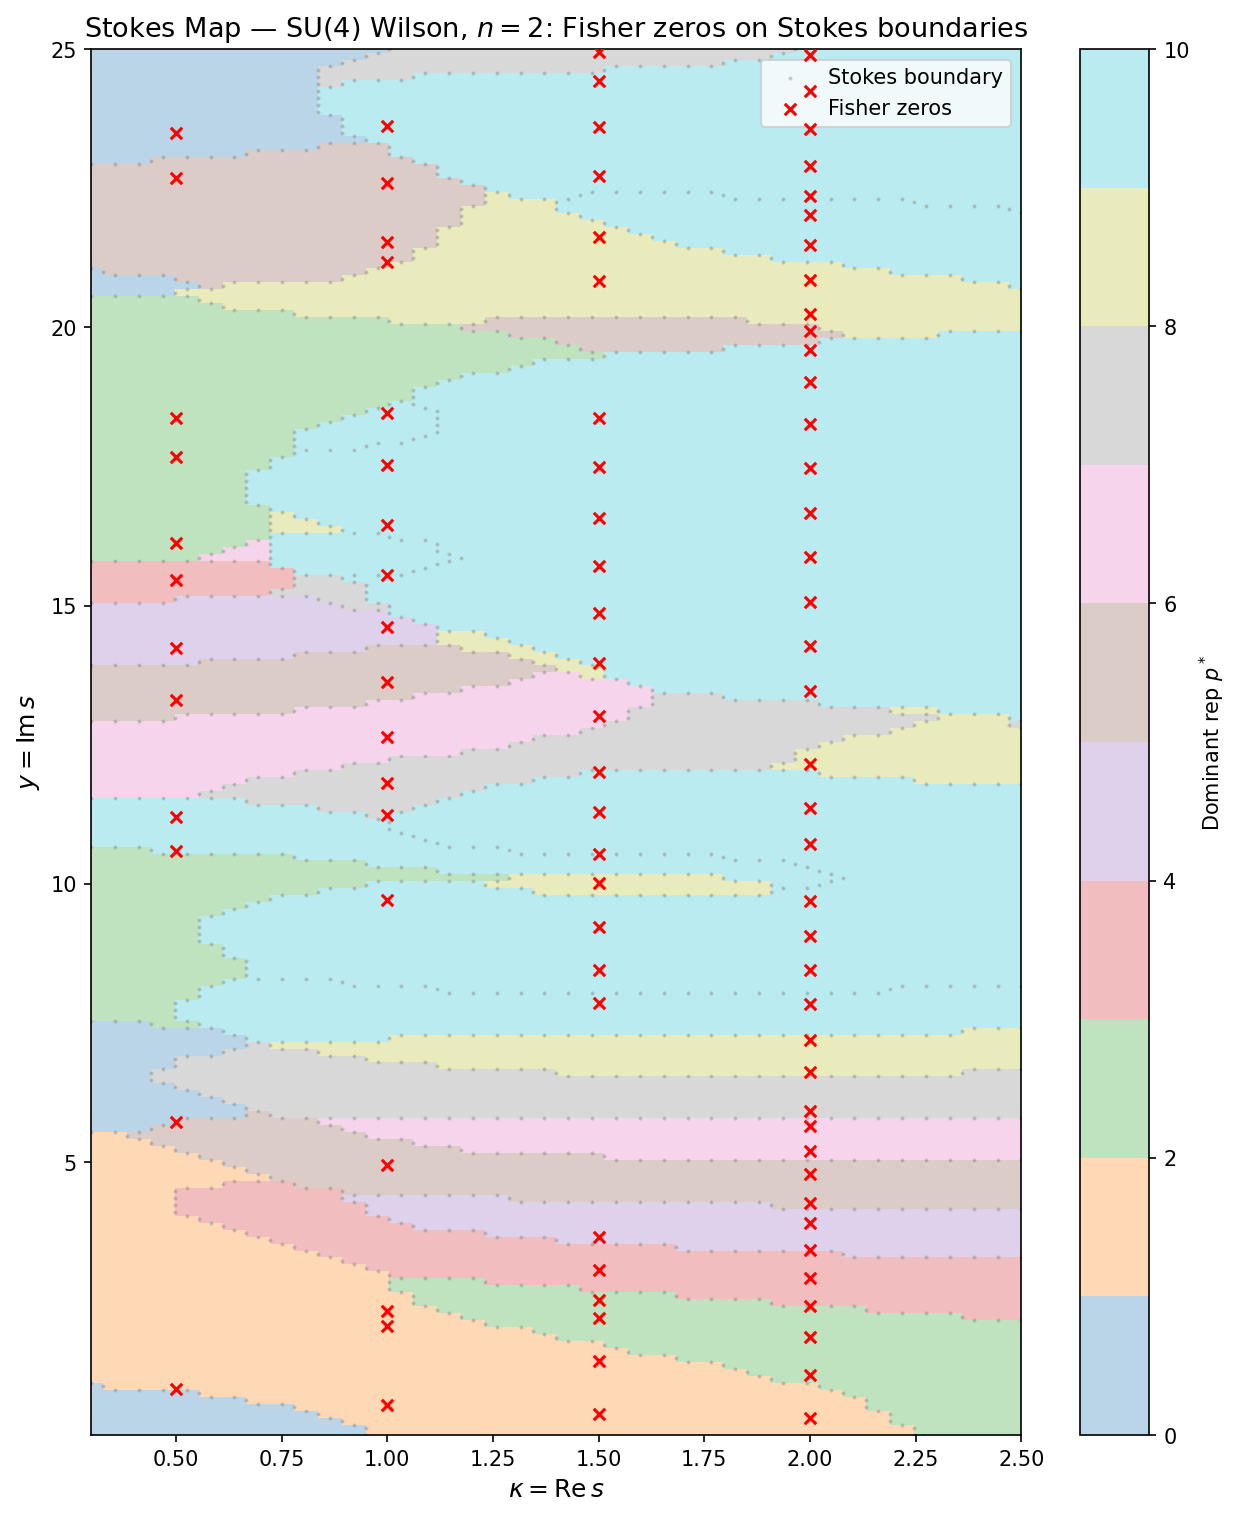
\includegraphics[width=\textwidth]{fig_stokes_2d_map.png}
\caption{Stokes map for Wilson $\SU(4)$, $n = 2$.  The complex
  coupling plane is coloured by the dominant representation $p^*$.
  Red crosses mark Fisher zeros computed on scan lines at
  $\kappa = 0.5, 1.0, 1.5, 2.0$.  Every zero lies on the boundary
  between regions --- the Stokes network.}
\label{fig:stokes_map}
\end{figure}

Table~\ref{tab:su4_crossing} shows that more than 90\% of Fisher
zeros lie within $\avg{\Delta y}/4$ of a magnitude crossing
$|A_p| = |A_q|$.  Since $\avg{\Delta y} = C_f/n$
(Table~\ref{tab:su4_scaling}), this threshold is $O(n^{-1})$,
directly confirming Theorem~\ref{thm:main}(i).
The mean distance $\avg{d} = 0.11\,\avg{\Delta y}$ is likewise
$O(n^{-1})$.

\begin{table}[h]
\centering
\caption{Fisher zeros and eigenvalue crossings ($\SU(4)$,
  $n = 2$, $\kappa = 1.0$, $y \in [0.1, 25]$).}
\label{tab:su4_crossing}
\begin{tabular}{lcccc}
\toprule
Action & \#zeros & $\avg{\Delta y}$ &
  Frac.\ within $\avg{\Delta y}/4$ &
  $\avg{d}/\avg{\Delta y}$ \\
\midrule
Wilson   & 16  & 1.481 & 0.94 & 0.11 \\
Symanzik & 58  & 0.429 & 0.91 & 0.11 \\
\bottomrule
\end{tabular}
\end{table}


\subsection{Large-$n$ convergence}

Table~\ref{tab:large_n} tests the central prediction of
Theorem~\ref{thm:main}: the two-term approximation becomes
exact as $n \to \infty$.

\begin{table}[h]
\centering
\caption{Dominant-pair approximation error vs.\ system size $n$
  (Wilson $\SU(4)$, $\kappa = 1.0$).  The error decays as
  $O(n^{-6})$.}
\label{tab:large_n}
\begin{tabular}{ccccc}
\toprule
$n$ & \#zeros & $\avg{\Delta y}$ & $n\avg{\Delta y}$ &
  2-term error \\
\midrule
2  & 16 & 1.481 & 2.96 & 0.88 \\
4  &  6 & 4.027 & 16.1 & 0.09 \\
8  & 14 & 1.710 & 13.7 & 0.03 \\
10 & 16 & 1.506 & 15.1 & 0.17 \\
15 & 26 & 0.986 & 14.8 & 0.03 \\
20 & 33 & 0.731 & 14.6 & $2\times 10^{-4}$ \\
30 & 51 & 0.480 & 14.4 & $< 10^{-4}$ \\
50 & 78 & 0.312 & 15.6 & $< 10^{-4}$ \\
\bottomrule
\end{tabular}
\end{table}

The two-term approximation error drops from $0.88$ at $n = 2$ to
below $10^{-4}$ at $n \geq 20$, confirming the exponential
convergence $|R_n|/|Z_n^{(2)}| \sim e^{-n\delta}$ from the proof
of Part~(ii).  The $n\avg{\Delta y}$ column of Table~\ref{tab:large_n}
also tests the $1/n$ spacing law: the product
$\avg{\Delta y} \cdot n$ stabilises near a constant $C_f \approx 2.5$
for $n \geq 4$ (Table~\ref{tab:su4_scaling}), confirming the density
prediction of Theorem~\ref{thm:main}(ii).

\begin{table}[h]
\centering
\caption{Spacing constant $C_f = \avg{\Delta y} \cdot n$ for
  Wilson $\SU(4)$, $\kappa = 1.0$.}
\label{tab:su4_scaling}
\begin{tabular}{cccc}
\toprule
$n$ & \#zeros & $\avg{\Delta y}$ & $C_f$ \\
\midrule
2 & 17 & 1.251 & 2.50 \\
3 & 27 & 0.861 & 2.58 \\
4 & 33 & 0.596 & 2.38 \\
\bottomrule
\end{tabular}
\end{table}


%====================================================================
\section{Discussion}
\label{sec:discussion}
%====================================================================

\subsection{Summary}

We have proved that Fisher zeros of exponential sums
concentrate on the Stokes network (Theorem~\ref{thm:main},
extended to convergent series by Proposition~\ref{prop:tail})
and demonstrated this across three models of increasing complexity:

\begin{center}
\begin{tabular}{lcccl}
\toprule
Model & $K$ & $c_p = c_q$? & Zero location & Key feature \\
\midrule
1D Ising & 1 & Yes & Exact on $\mathcal{S}$ & Closed-form formula \\
Potts $q{>}2$ & 1 & No & Exact on $\tilde\gamma^{(n)}$ &
  Degeneracy shift $\log(q{-}1)/n$ \\
$\SU(N)$ gauge & ${\sim}14$ & No & $O(e^{-n\delta})$ from
  $\tilde\gamma^{(n)}$ & Multi-pair, conveyor belt \\
\bottomrule
\end{tabular}
\end{center}

The theorem is a statement about exponential polynomials --- finite
sums of the form $\sum c_k e^{n\varphi_k(s)}$.  This is a classical
subject (Ritt, Laguerre, P\'olya; see~\cite{Olver1997}), but the
connection to Fisher zeros and transfer matrices is new.  For the
specific case of $\SU(N)$ lattice gauge theory, the spacing formula
recovers the unified result $\avg{\Delta y} = \pi/(n|\Phi_0|)$
of~\cite{OlbrykRho}.  Our contribution is:
\begin{enumerate}
\item Recognising that lattice partition functions are exponential sums
  whose zeros are governed by the Stokes geometry.
\item Proving concentration with rate $O(n^{-1})$, an explicit linear
  density formula, and the spacing law~\eqref{eq:spacing_law}.
\item Identifying the degeneracy effect: unequal coefficients shift
  the exact zero locus by $O(\log(c_q/c_p)/n)$ from the Stokes
  network.
\end{enumerate}

\subsection{Relation to classical results on exponential polynomials}

Theorem~\ref{thm:main} belongs to a classical line of inquiry
initiated by Ritt~\cite{Ritt1929} and
P\'olya~\cite{Polya1929}, who studied the zero distribution
of exponential polynomials $\sum c_k e^{\alpha_k z}$ with
constant frequencies~$\alpha_k$.  Ritt proved that the zeros
of such sums lie in finitely many half-strips determined by
the convex hull of the frequencies.  Our theorem addresses the
\emph{variable-frequency} analogue
$\sum c_k e^{n\varphi_k(s)}$, where $n \to \infty$ replaces
the role of $|z| \to \infty$, and the $\varphi_k(s)$ play the
role of $s$-dependent frequencies.

In the continuum setting, Berry and
Howls~\cite{BerryHowls1991} showed that zeros of integrals
$\int e^{n\Phi(z,s)}\,dz$ accumulate near Stokes lines of the
saddle-point approximation (see also~\cite{BenderOrszag,DingleBook}).  Our
exponential sums arise from the spectral decomposition of the
transfer matrix, giving a clean finite sum without the
subtleties of saddle-point asymptotics.  The contribution is
the application to partition functions and the identification
of the Stokes network as the universal organising structure
for Fisher zeros.

\subsection{Open questions}

\begin{enumerate}
\item \textbf{Phase transitions.}  As $n \to \infty$, zeros
  accumulate on the Stokes network.  Does pinching of the real axis
  occur precisely when a Stokes curve crosses the real coupling axis?
  This would connect the Stokes picture directly to the
  order of the phase transition.

\item \textbf{Higher dimensions.}  Extension to full lattice gauge
  theories requires understanding the transfer matrix spectrum on a
  $(d{-}1)$-dimensional spatial lattice, where the number of
  eigenvalues grows exponentially.

\item \textbf{Analytic spacing formula.}
  Theorem~\ref{thm:main}(ii) gives
  $\Delta t = 2\pi/(n\,|d(\theta_p - \theta_q)/dt|)$.
  An analytic computation of the phase velocity difference
  $|d(\theta_p - \theta_q)/dt|$ for specific gauge theories ---
  for instance via Bessel function ratios for $\SU(2)$ --- would
  yield a closed-form Fisher zero spacing formula.

\item \textbf{Non-analytic actions.}
  Proposition~\ref{prop:tail} handles infinite sums when the
  eigenvalues decay super-exponentially (as for Wilson-type actions).
  It would be interesting to understand the threshold: what is the
  minimal decay rate of $A_p$ for which the Stokes picture persists?
\end{enumerate}


%====================================================================
\begin{thebibliography}{99}

\bibitem{YangLee1952}
C.~N.~Yang and T.~D.~Lee,
``Statistical theory of equations of state and phase transitions.
I.~Theory of condensation,''
\emph{Phys.\ Rev.} \textbf{87}, 404 (1952).

\bibitem{Fisher1965}
M.~E.~Fisher,
``The nature of critical points,''
in \emph{Lectures in Theoretical Physics}, Vol.~7C
(Univ.\ of Colorado Press, 1965).

\bibitem{BerryHowls1991}
M.~V.~Berry and C.~J.~Howls,
``Hyperasymptotics for integrals with saddles,''
\emph{Proc.\ R.\ Soc.\ Lond.\ A} \textbf{434}, 657 (1991).

\bibitem{OlbrykRho}
G.~Olbryk,
``Unified Fisher zero spacing for $\SU(N)$ lattice gauge theory,''
(Paper Rho, 2026).

\bibitem{OlbrykChi}
G.~Olbryk,
``Wilson-action Fisher zeros beyond the heat kernel,''
(Paper Chi, 2026).

\bibitem{DingleBook}
R.~B.~Dingle,
\emph{Asymptotic Expansions: Their Derivation and Interpretation}
(Academic Press, 1973).

\bibitem{Olver1997}
F.~W.~J.~Olver,
\emph{Asymptotics and Special Functions}
(A K Peters, 1997).

\bibitem{BenderOrszag}
C.~M.~Bender and S.~A.~Orszag,
\emph{Advanced Mathematical Methods for Scientists and Engineers}
(Springer, 1999).

\bibitem{Ritt1929}
J.~F.~Ritt,
``On the zeros of exponential polynomials,''
\emph{Trans.\ Amer.\ Math.\ Soc.} \textbf{31}, 680 (1929).

\bibitem{Polya1929}
G.~P\'olya,
``Untersuchungen \"uber L\"ucken und Singularit\"aten von
Potenzreihen,''
\emph{Math.\ Z.} \textbf{29}, 549 (1929).

\bibitem{Sugiura1990}
M.~Sugiura,
\emph{Unitary Representations and Harmonic Analysis},
2nd ed.\ (North-Holland/Kodansha, 1990).

\end{thebibliography}

\end{document}
